\documentclass{article}[a4paper]
\usepackage{tcolorbox}
\usepackage[pdfborder={0 0 0}]{hyperref}
\usepackage{tabularx}
\usepackage{enumitem}
\usepackage{graphicx}

\makeatletter
\newcommand\subsubsubsection{\@startsection{paragraph}{4}{\z@}%
            {-2.5ex\@plus -1ex \@minus -.25ex}%
            {1.25ex \@plus .25ex}%
            {\normalfont\normalsize\bfseries}}
\makeatother
\setcounter{secnumdepth}{4}
\setcounter{tocdepth}{4}

\title{SWT21 lab kit \\ User manual}
\author{Binäs Teknik AB}

\begin{document}
\maketitle
\tableofcontents
\newpage

\section{General}

The SWT21 lab kit allows communication and measurements using a single
microcontroller with a carrier board. The lab kit runs a firmware allowing a
computer to be connected as host which can then control the lab kit using the
host interface. This allows us to inspect network communication, interact with
hardware, etc. from the host computer.

The general connectivity of the lab kit is

\medskip
\renewcommand{\arraystretch}{1.5}
\noindent
\begin{tabularx}{\textwidth}{|p{2cm}|p{1.5cm}|X|}
\hline
test & test & Comment \\
\hline
WiFi \hbox{802.11 b/g/n} 2.4 GHz &  & AP mode and STA mode \\
\hline
Bluetooth 4.2 & &  Classic \& Low energy mode \\
\hline
CAN 2.0 & 1x & Only standard ID:s, 120 $\Omega$ termination available via jumper
 configuration \\
\hline
LIN 2.2 & 1x & Master or slave via jumper configuration \\
\hline
UART & 1x & 3.3V maximum 2 Mbit/s, configurable 1-2 stop bits and parity bit \\
\hline
ADC & 2x & 0-3 V or 0-30 V via jumper configuration \\
\hline
DAC & 2x & 0-3 V or 0-12 V via jumper configuration (0-12 V) requires external power supply)\\
\hline
\end{tabularx}


\subsection{Syntax rules}
This manual uses the following syntax for describing commands

\medskip
\noindent
\begin{tabularx}{\textwidth}{|p{4cm}|X|}
\hline
<text> & indicates option to be replaced by other text \\
\hline
[text] & optional argument to be replaced by other text if used\\
\hline
[text]... or <text>... & indicates multiple arguments may be used \\
\hline
\{a|b\} & means either a or b may be used \\
\hline
\end{tabularx}

\section{Hardware layout}

\begin{center}
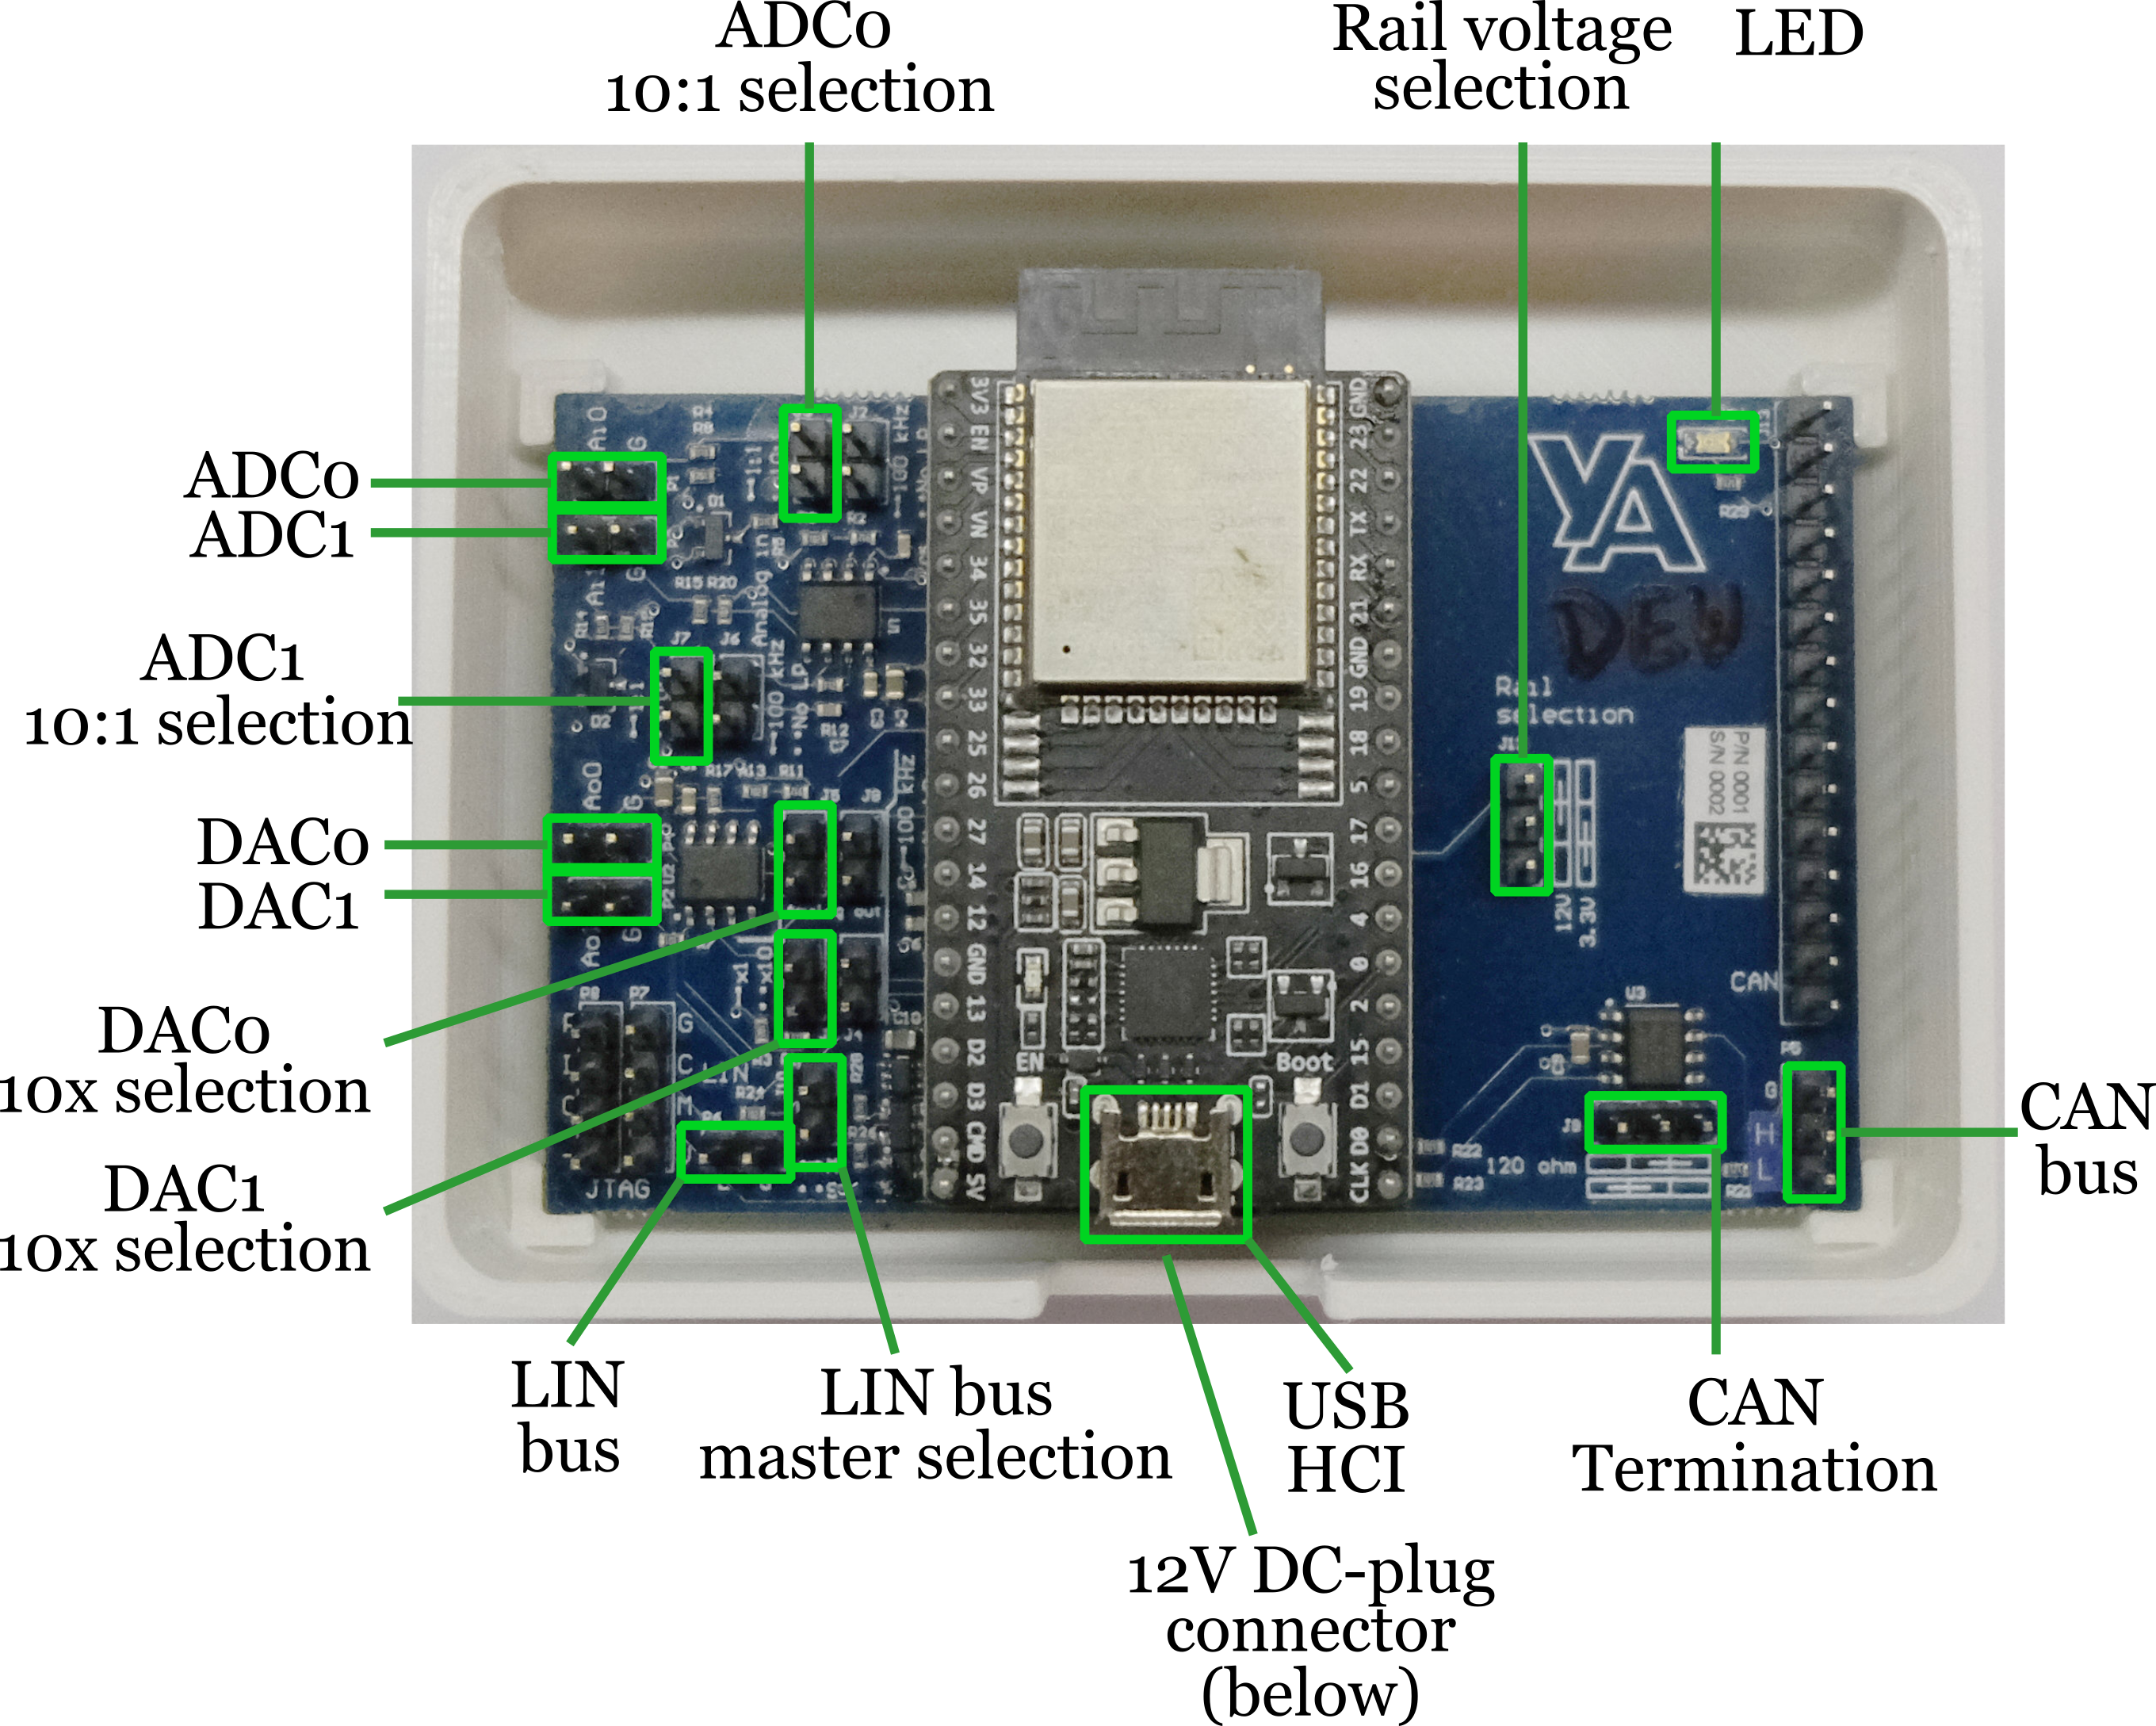
\includegraphics[width=10cm]{lab-pcb-connections.png}
\end{center}

\section{Host interface}
%configuration
%what is unsolicited commands
%syntax

The device is connected to a computer via USB. This connection provides a
USB-UART interface which presents itself as a serial port on the computer,
(COM3, /dev/ttyUSBx, or similar).

The HCI on the lab kit is preconfigured to

\medskip
\noindent
\begin{tabularx}{\textwidth}{|p{3cm}|X|}
\hline
Baudrate: & 2 Mbit/s \\
\hline
Stopbits: & 1 \\
\hline
Parity: & None \\
\hline
\end{tabularx}

To access the HCI you may use any serial port monitor of your choice, one
recommended monitor is miniterm which is part of the pyserial Python package. To
use it follow these steps in the command prompt/terminal:

\begin{enumerate}
\item Run \texttt{pip3 install pyserial}
\item Run \texttt{python -m serial.tools.miniterm <COM-port> 2000000} where
      <COM-port> is replaced with the actual COM port, e.g. COM3.
\end{enumerate}

\subsection{System requirements}

The lab kit requires a computer with an USB port and is compatible with Windows,
MacOS and Linux.

Drivers for the USB-UART bridge are available from
\url{https://www.silabs.com/developers/usb-to-uart-bridge-vcp-drivers}

\subsection{Protocol}

The communication interface uses text-based communication where each line is a
command or a response. Each line may be up to 255 bytes and ends with a new
line control character
(\textbackslash n). Other control characters will be ignored. The format of
the commands is as follows:
\begin{verbatim}
<module> <command> [arguments]...
e.g.: CAN config filter1 1f0 f70
\end{verbatim}

Responses can either be acknowledged with an
\begin{verbatim}
OK [data]
\end{verbatim}
, where data is any optional data returned by the command, or an error:
\begin{verbatim}
ERR <reason>
\end{verbatim}

General errors:
\begin{itemize}[noitemsep]
\item ERR Invalid command
\item ERR Invalid arguments
\item ERR Command too long
\end{itemize}

Unsolicited commands are events sent from the lab kit to the host without a
preceding command asking directly for it. It is used for events like incoming
communication packets and periodic measurment data. The syntax is the same as
for commands but no response is expected.

\subsubsection{Boot}
On boot an informational string will be written on the host interface with
the following syntax

\begin{verbatim}
SWT21 lab kit
Booting...
Firmware version: <fw version>
Boot reason: <reason>
\end{verbatim}

<reason> may be due to several reasons:
\begin{itemize}[noitemsep]
\item Power on
\item SW reset
\item WDT reset
\item Brownout
\item OS panic
\item Unknown
\end{itemize}

\section{Firmware update}
To update the firmware download and install esptool from the official Python
repository (Python is required to be installed).

Steps:
\begin{enumerate}
\item Start a command prompt/terminal.
\item Run "pip3 install esptool" to install esptool.
\item Run \texttt{esptool.py --chep esp32 --port <port> --baud 921600 write\_flash 0x10000 <firmware.bin>} (where <port> is the port in use, e.g. COM3, and <firmware.bin> is your firmware file, e.g. v1.1.bin)
\item Press the EN and the Boot buttons on the lab kit, then release first the EN
      button and then the Boot button.
\item If the flash counter does not start retry the last step again.
\end{enumerate}

\section{LED}
The LED can be used to control the LED on the board which may be used to
identify which board is currently connected.

\subsection{LED commands}
\subsubsection{led help}
\begin{tcolorbox}
	{\bf Syntax}

	\parshape 1 1cm \dimexpr\linewidth-2cm\relax
	led help

	\medskip
	{\bf Description}

	\parshape 1 1cm \dimexpr\linewidth-2cm\relax
	This command prints out a summary of the LED commands.

	\medskip
	{\bf Return values}

	\parshape 1 1cm \dimexpr\linewidth-2cm\relax
	OK \\
	<help text>
\end{tcolorbox}

\subsubsection{led \{on|off\}}
\begin{tcolorbox}
	{\bf Syntax}

	\parshape 1 1cm \dimexpr\linewidth-2cm\relax
	led \{on|off\}

	\medskip
	{\bf Description}

	\parshape 1 1cm \dimexpr\linewidth-2cm\relax
	This command turns the LED on or off.
	Default state is off.

	\medskip
	{\bf Return values}

	\parshape 1 1cm \dimexpr\linewidth-2cm\relax
	OK
\end{tcolorbox}

\subsubsection{led blink [half period]}
\begin{tcolorbox}
	{\bf Syntax}

	\parshape 1 1cm \dimexpr\linewidth-2cm\relax
	led blink [half period]

	\medskip
	{\bf Description}

	\parshape 1 1cm \dimexpr\linewidth-2cm\relax
	This command starts blinking the LED staying on and off for half period
	milliseconds. If ommited the default time of 500 ms is used.
	\medskip \\
	{\it half period} - the time spent in on or off state respectively in milliseconds \\

	\medskip
	{\bf Return values}

	\parshape 1 1cm \dimexpr\linewidth-2cm\relax
	OK
\end{tcolorbox}

\section{CAN}
The CAN bus can be used to send and recive 11-bit ID CAN frames.
When sending frames they can only be sent as single frames. Single frames are
enqueued on the transmit buffer immediately after a "can send" command has been sent.

\subsection{CAN commands}
\subsubsection{can help}
\begin{tcolorbox}
	{\bf Syntax}

	\parshape 1 1cm \dimexpr\linewidth-2cm\relax
	can help

	\medskip
	{\bf Description}

	\parshape 1 1cm \dimexpr\linewidth-2cm\relax
	This command prints out a summary of the CAN commands.

	\medskip
	{\bf Return values}

	\parshape 1 1cm \dimexpr\linewidth-2cm\relax
	OK \\
	<help text>
\end{tcolorbox}

\subsubsection{can rx}
\begin{tcolorbox}
	{\bf Syntax}

	\parshape 1 1cm \dimexpr\linewidth-2cm\relax
	can rx \{on|off\}

	\medskip
	{\bf Description}

	\parshape 1 1cm \dimexpr\linewidth-2cm\relax
	This command enables or disables receiving CAN frames. When off no unsolicited
	CAN frame commands will be sent. \\
	Default state is off.

	\medskip
	{\bf Return values}

	\parshape 1 1cm \dimexpr\linewidth-2cm\relax
	OK
\end{tcolorbox}

\subsubsection{can send}
\begin{tcolorbox}
	{\bf Syntax}

	\parshape 1 1cm \dimexpr\linewidth-2cm\relax
	can send <can\_id>\#\{R|data\}

	\medskip
	{\bf Description}

	\parshape 1 1cm \dimexpr\linewidth-2cm\relax
	This command sends a single CAN frame on the CAN bus. On insufficient CAN
	memory it will return an overflow error.
	\medskip \\
	{\it can\_id} - the CAN ID in hexadecimal \\
	{\it R} - represents a remote frame \\
	{\it data} - is the frame data in hexadecimal \\
	\medskip \\
	Example: \texttt{can send 13f\#02e8}

	\medskip
	{\bf Return values}

	\parshape 1 1cm \dimexpr\linewidth-2cm\relax
	OK \\
	ERR Invalid argument \\
	ERR Overflow
\end{tcolorbox}

\subsubsection{can config}
\begin{tcolorbox}
	{\bf Syntax}

	\parshape 1 1cm \dimexpr\linewidth-2cm\relax
	can config <config key> [<arg>]

	\medskip
	{\bf Description}

	\parshape 1 1cm \dimexpr\linewidth-2cm\relax
	This command sets the configuration values of the CAN subsystem.
	Leaving out an argument returns the current value(s) with the same argument
	format.

	\medskip
	{\bf Return values}

	\parshape 1 1cm \dimexpr\linewidth-2cm\relax
	OK \\
	OK <value>... \\
	ERR Invalid argument
\end{tcolorbox}

\subsubsubsection{can config brp}
\begin{tcolorbox}
	{\bf Config key}

	\parshape 1 1cm \dimexpr\linewidth-2cm\relax
	baudrate

	\medskip
	{\bf Arguments}

	\parshape 1 1cm \dimexpr\linewidth-2cm\relax
	<brp> - CAN clock baudrate prescaler

	\medskip
	{\bf Description}

	\parshape 1 1cm \dimexpr\linewidth-2cm\relax
	This configuration sets the CAN baudrate prescaler. The final baudrate can
	be calculated from \vspace{2mm} \\
	\fbox{$\textrm{can bitrate} = \frac{80 000 000}{brp * (1 + tseg\_1 + tseg\_2)}$}
\end{tcolorbox}

\subsubsubsection{can config tseg\_1}
\begin{tcolorbox}
	{\bf Config key}

	\parshape 1 1cm \dimexpr\linewidth-2cm\relax
	tseg\_1

	\medskip
	{\bf Arguments}

	\parshape 1 1cm \dimexpr\linewidth-2cm\relax
	<tseg\_1> - CAN time segment 1

	\medskip
	{\bf Description}

	\parshape 1 1cm \dimexpr\linewidth-2cm\relax
	This configuration sets the number of time quantas for CAN tseg\_1. The final baudrate can
	be calculated from \vspace{2mm} \\
	\fbox{$\textrm{can bitrate} = \frac{80 000 000}{brp * (1 + tseg\_1 + tseg\_2)}$}
\end{tcolorbox}

\subsubsubsection{can config tseg\_2}
\begin{tcolorbox}
	{\bf Config key}

	\parshape 1 1cm \dimexpr\linewidth-2cm\relax
	tseg\_2

	\medskip
	{\bf Arguments}

	\parshape 1 1cm \dimexpr\linewidth-2cm\relax
	<tseg\_2> - CAN time segment 2

	\medskip
	{\bf Description}

	\parshape 1 1cm \dimexpr\linewidth-2cm\relax
	This configuration sets the number of time quantas for CAN tseg\_2. The final baudrate can
	be calculated from \vspace{2mm} \\
	\fbox{$\textrm{can bitrate} = \frac{80 000 000}{brp * (1 + tseg\_1 + tseg\_2)}$}
\end{tcolorbox}

\subsubsubsection{can config sjw}
\begin{tcolorbox}
	{\bf Config key}

	\parshape 1 1cm \dimexpr\linewidth-2cm\relax
	sjw

	\medskip
	{\bf Arguments}

	\parshape 1 1cm \dimexpr\linewidth-2cm\relax
	<sjw> - CAN synchronization jump width

	\medskip
	{\bf Description}

	\parshape 1 1cm \dimexpr\linewidth-2cm\relax
	This configuration sets the CAN synchronization jump width. This is the
	maximum number of time quantas that the synchronization may be synchronized.
\end{tcolorbox}

\subsection{Unsolicited CAN commands}

\subsubsection{CAN RX}
\begin{tcolorbox}
	{\bf Syntax}

	\parshape 1 1cm \dimexpr\linewidth-2cm\relax
	CAN RX: <can\_id>\#\{R|data\}

	\medskip
	{\bf Description}

	\parshape 1 1cm \dimexpr\linewidth-2cm\relax
	This command is sent when the system receives a CAN frame including its data
	\medskip \\
	{\it can\_id} - the CAN ID in hexadecimal \\
	{\it R} - represents a remote frame \\
	{\it data} - is the frame data in hexadecimal

	\medskip
	Example: \texttt{CAN RX: 74e\#8e98}
\end{tcolorbox}

\section{LIN}

The LIN bus can be used to send and recive LIN 2.2 frames.
When sending frames they can only be sent as single frames. Single frames are
enqueued on the transmit buffer immediately after a "lin single" command has been sent.


\subsection{LIN commands}
\subsubsection{lin help}
\begin{tcolorbox}
	{\bf Syntax}

	\parshape 1 1cm \dimexpr\linewidth-2cm\relax
	lin help

	\medskip
	{\bf Description}

	\parshape 1 1cm \dimexpr\linewidth-2cm\relax
	This command prints out a summary of the LIN commands.

	\medskip
	{\bf Return values}

	\parshape 1 1cm \dimexpr\linewidth-2cm\relax
	OK \\
	<help text>
\end{tcolorbox}

\subsubsection{lin txbuf}
\begin{tcolorbox}
	{\bf Syntax}

	\parshape 1 1cm \dimexpr\linewidth-2cm\relax
	lin txbuf <id>\#<data>

	\medskip
	{\bf Description}

	\parshape 1 1cm \dimexpr\linewidth-2cm\relax
	This command loads <data> into the send buffer for <id>.
	\medskip \\
	{\it id} - the LIN ID in decimal \\
	{\it data} - is the frame data in hexadecimal \\
	\medskip \\
	Example: \texttt{lin txbuf 17\#02e8}

	\medskip
	{\bf Return values}

	\parshape 1 1cm \dimexpr\linewidth-2cm\relax
	OK \\
	ERR Invalid argument
\end{tcolorbox}

\subsubsection{lin single}
\begin{tcolorbox}
	{\bf Syntax}

	\parshape 1 1cm \dimexpr\linewidth-2cm\relax
	lin single <id>

	\medskip
	{\bf Description}

	\parshape 1 1cm \dimexpr\linewidth-2cm\relax
	This command enques sending out a frame header for <id>. This command should
	only be run on the LIN master.
	\medskip \\
	{\it id} - the LIN ID in decimal \\

	\medskip
	{\bf Return values}

	\parshape 1 1cm \dimexpr\linewidth-2cm\relax
	OK
\end{tcolorbox}

\subsubsection{lin config}
\begin{tcolorbox}
	{\bf Syntax}

	\parshape 1 1cm \dimexpr\linewidth-2cm\relax
	lin config <config key> [<arg>]

	\medskip
	{\bf Description}

	\parshape 1 1cm \dimexpr\linewidth-2cm\relax
	This command sets the configuration values of the LIN subsystem.
	Leaving out an argument returns the current value(s) with the same argument
	format.

	\medskip
	{\bf Return values}

	\parshape 1 1cm \dimexpr\linewidth-2cm\relax
	OK \\
	OK <value>... \\
	ERR Invalid argument
\end{tcolorbox}

\subsubsubsection{lin config rx [<id> <len> <chks-type>] | off]}
\begin{tcolorbox}
	{\bf Config key}

	\parshape 1 1cm \dimexpr\linewidth-2cm\relax
	rx [\{<id> <len> <chks-type>] | off\}]

	\medskip
	{\bf Arguments}

	\parshape 1 1cm \dimexpr\linewidth-2cm\relax
	<id> - LIN frame id \\
	<len> - LIN frame len \\
	<chks-type> - LIN frame checksum type (0: classic, 1: enhanced)

	\medskip
	{\bf Description}

	\parshape 1 1cm \dimexpr\linewidth-2cm\relax
	This configuration sets the configuration for a LIN frame to receive by this
	node. Using the off key will disable receiving this LIN frame.
\end{tcolorbox}

\subsubsubsection{lin config tx [<id> <len> <chks-type>] | off]}
\begin{tcolorbox}
	{\bf Config key}

	\parshape 1 1cm \dimexpr\linewidth-2cm\relax
	tx [\{<id> <len> <chks-type>] | off\}]

	\medskip
	{\bf Arguments}

	\parshape 1 1cm \dimexpr\linewidth-2cm\relax
	<id> - LIN frame id \\
	<len> - LIN frame len \\
	<chks-type> - LIN frame checksum type (0: classic, 1: enhanced)

	\medskip
	{\bf Description}

	\parshape 1 1cm \dimexpr\linewidth-2cm\relax
	This configuration sets the configuration for a LIN frame to transmitt by this
	node. Using the off key will disable transmitting this LIN frame.
\end{tcolorbox}

\subsection{Unsolicited LIN commands}

\subsubsection{LIN RX}
\begin{tcolorbox}
	{\bf Syntax}

	\parshape 1 1cm \dimexpr\linewidth-2cm\relax
	LIN RX: <id>\#<data>

	\medskip
	{\bf Description}

	\parshape 1 1cm \dimexpr\linewidth-2cm\relax
	This command is sent when the system receives a LIN frame.
	\medskip \\
	{\it id} - the LIN ID in decimal \\
	{\it data} - is the frame data in hexadecimal

	\medskip
	Example: \texttt{LIN RX: 13\#0e12}
\end{tcolorbox}

\section{UART}

The UART can be used to send and recive UART characters.


\subsection{UART commands}
\subsubsection{uart help}
\begin{tcolorbox}
	{\bf Syntax}

	\parshape 1 1cm \dimexpr\linewidth-2cm\relax
	uart help

	\medskip
	{\bf Description}

	\parshape 1 1cm \dimexpr\linewidth-2cm\relax
	This command prints out a summary of the UART commands.

	\medskip
	{\bf Return values}

	\parshape 1 1cm \dimexpr\linewidth-2cm\relax
	OK \\
	<help text>
\end{tcolorbox}

\subsubsection{uart sendline}
\begin{tcolorbox}
	{\bf Syntax}

	\parshape 1 1cm \dimexpr\linewidth-2cm\relax
	uart sendline <text>

	\medskip
	{\bf Description}

	\parshape 1 1cm \dimexpr\linewidth-2cm\relax
	This command sends <text> over UART and ends with a newline character '\textbackslash n'.
	\medskip \\
	{\it text} - the line of text to send \\

	\medskip
	Example: \texttt{uart sendline Hello world!}

	\medskip
	{\bf Return values}

	\parshape 1 1cm \dimexpr\linewidth-2cm\relax
	OK \\
	ERR Invalid argument
\end{tcolorbox}

\subsubsection{uart config}
\begin{tcolorbox}
	{\bf Syntax}

	\parshape 1 1cm \dimexpr\linewidth-2cm\relax
	uart config <config key> [<arg>]

	\medskip
	{\bf Description}

	\parshape 1 1cm \dimexpr\linewidth-2cm\relax
	This command sets the configuration values of the UART subsystem.
	Leaving out an argument returns the current value(s) with the same argument
	format.

	\medskip
	{\bf Return values}

	\parshape 1 1cm \dimexpr\linewidth-2cm\relax
	OK \\
	OK <value>... \\
	ERR Invalid argument
\end{tcolorbox}

\subsubsubsection{uart config baudrate [<baudrate>]}
\begin{tcolorbox}
	{\bf Config key}

	\parshape 1 1cm \dimexpr\linewidth-2cm\relax
	config baudrate [<baudrate>]

	\medskip
	{\bf Arguments}

	\parshape 1 1cm \dimexpr\linewidth-2cm\relax
	<baudrate> - UART baudrate

	\medskip
	{\bf Description}

	\parshape 1 1cm \dimexpr\linewidth-2cm\relax
	This configuration sets the baudrate for the UART for both transmitting and
	receiving.
\end{tcolorbox}

\subsubsubsection{uart config parity [<parity>]}
\begin{tcolorbox}
	{\bf Config key}

	\parshape 1 1cm \dimexpr\linewidth-2cm\relax
	config parity [<parity>]

	\medskip
	{\bf Arguments}

	\parshape 1 1cm \dimexpr\linewidth-2cm\relax
	<parity> - UART parity, (n: none, e: even, o: odd)

	\medskip
	{\bf Description}

	\parshape 1 1cm \dimexpr\linewidth-2cm\relax
	This configuration sets the parity for the UART for both transmitting and
	receiving.

	\medskip
	Example: \texttt{uart config parity e} will set even parity
\end{tcolorbox}


\subsubsubsection{uart config stopbits [<stopbits>]}
\begin{tcolorbox}
	{\bf Config key}

	\parshape 1 1cm \dimexpr\linewidth-2cm\relax
	config stopbits [<stopbits>]

	\medskip
	{\bf Arguments}

	\parshape 1 1cm \dimexpr\linewidth-2cm\relax
	<stopbits> - UART stopbits

	\medskip
	{\bf Description}

	\parshape 1 1cm \dimexpr\linewidth-2cm\relax
	This configuration sets the number of stopbits for the UART for both transmitting and
	receiving.
\end{tcolorbox}

\subsection{Unsolicited UART commands}

\subsubsection{UART}
\begin{tcolorbox}
	{\bf Syntax}

	\parshape 1 1cm \dimexpr\linewidth-2cm\relax
	UART: <byte>

	\medskip
	{\bf Description}

	\parshape 1 1cm \dimexpr\linewidth-2cm\relax
	This command is sent when the system receives a byte on UART.
	\medskip \\
	{\it byte} - the byte received, hexadecimal if < 0x20, otherwise printed as ASCII.

	\medskip
	Example: \texttt{UART: 0x0a} \\
	Example: \texttt{UART: H}
\end{tcolorbox}

\section{ADC}

The ADC can be used to measure voltages, both static and dynamic. It can take
either single measures or using triggers to take many measuremnts around a
trigger condition. Two channels are available
which can be accessed using \texttt{adc0} or \texttt{adc1}.

Each channel may be configured in hardware using jumpers to either use 1:1
voltage scaling with an input voltage range of 0-3 V or 10:1 scaling with a
voltage range of 0-30 V.

Values from the ADC may either be a floating point value in volts or a raw ADC
conversion value from the ADC in hexadecimal.

The submodule uses the following calibration values for converting raw ADC values to
voltages using a linear mapping.

\medskip

\noindent
\begin{tabularx}{\textwidth}{|p{4cm}|X|}
\hline
Calibration variable & Description \\
\hline
adc<n>\_v1x\_0\_2v & the measured raw ADC value when applying 0.2 V to the
ADC configured in 1:1 voltage division. \\
\hline
adc<n>\_v1x\_2v & the measured raw ADC value when applying 2 V to the
ADC configured in 1:1 voltage division. \\
\hline
adc<n>\_v10x\_2v & the measured raw ADC value when applying 2 V to the
ADC configured in 10:1 voltage division. \\
\hline
adc<n>\_v10x\_20v & the measured raw ADC value when applying 20 V to the
ADC configured in 10:1 voltage division. \\
\hline
\end{tabularx}

\subsection{ADC commands}
\subsubsection{adc<n> help}
\begin{tcolorbox}
	{\bf Syntax}

	\parshape 1 1cm \dimexpr\linewidth-2cm\relax
	adc<n> help

	\medskip
	{\bf Description}

	\parshape 1 1cm \dimexpr\linewidth-2cm\relax
	This command prints out a summary of the ADC commands.

	\medskip
	{\bf Return values}

	\parshape 1 1cm \dimexpr\linewidth-2cm\relax
	OK \\
	<help text>
\end{tcolorbox}

\subsubsection{adc<n> off}
\begin{tcolorbox}
	{\bf Syntax}

	\parshape 1 1cm \dimexpr\linewidth-2cm\relax
	adc<n> off

	\medskip
	{\bf Description}

	\parshape 1 1cm \dimexpr\linewidth-2cm\relax
	This command disables all periodic readings. \\
	\medskip
	{\it n} - the ADC channel number, 0 or 1 \\
	\medskip
	Example: \texttt{acd0 off}

	\medskip
	{\bf Return values}

	\parshape 1 1cm \dimexpr\linewidth-2cm\relax
	OK
\end{tcolorbox}

\subsubsection{adc<n> single}
\begin{tcolorbox}
	{\bf Syntax}

	\parshape 1 1cm \dimexpr\linewidth-2cm\relax
	adc<n> single

	\medskip
	{\bf Description}

	\parshape 1 1cm \dimexpr\linewidth-2cm\relax
	This command performs a single ADC measurement and returns the value
	immediately. \\
	\medskip
	{\it n} - the ADC channel number, 0 or 1

	\medskip
	{\bf Return values}

	\parshape 1 1cm \dimexpr\linewidth-2cm\relax
	ADC<n> <value> \\
	{\it value} - the measured vaule, either in floating point or hexadecimal
	raw value
\end{tcolorbox}

\subsubsection{adc0 trig <trig value> <sample rate> <m> <n>}
\begin{tcolorbox}
	{\bf Syntax}

	\parshape 1 1cm \dimexpr\linewidth-2cm\relax
	adc0 trig <trig value> <sample rate> <m> <n>

	\medskip
	{\bf Description}

	\parshape 1 1cm \dimexpr\linewidth-2cm\relax
	This command is only available on ADC channel 0. \\
	This command performs a trigged measurement, it will continuosly monitor the
	ADC input for the trigger value and when it finds it it will store <m> number
	of samples before it and <n> numbers of samples after it and send it to the
	host.

	\medskip
	{\it trig value} - the raw trigger value in hexadecimal \\
	{\it sample rate} - the rate at which to sample the ADC in samples per second \\
	{\it m} - the number of values to output before the trigger value \\
	{\it n} - the number of values to output after the trigger value

	\medskip
	{\bf Return values}

	\parshape 1 1cm \dimexpr\linewidth-2cm\relax
	ADC0 clk: <clk> \\
	\medskip
	{\it <clk>} - The actual sample rate used by the ADC
\end{tcolorbox}

\subsubsection{adc0 trig off}
\begin{tcolorbox}
	{\bf Syntax}

	\parshape 1 1cm \dimexpr\linewidth-2cm\relax
	adc0 trig off

	\medskip
	{\bf Description}

	\parshape 1 1cm \dimexpr\linewidth-2cm\relax
	This command is only available on ADC channel 0. \\
	This command disables any currently running trigger condition.

	\medskip
	{\bf Return values}

	\parshape 1 1cm \dimexpr\linewidth-2cm\relax
	OK \\
\end{tcolorbox}

\subsubsection{adc<n> config}
\begin{tcolorbox}
	{\bf Syntax}

	\parshape 1 1cm \dimexpr\linewidth-2cm\relax
	adc<n> config <config key> [<arg>]

	\medskip
	{\bf Description}

	\parshape 1 1cm \dimexpr\linewidth-2cm\relax
	This command sets the configuration values of the ADC subsystem.
	Leaving out an argument returns the current value(s) with the same argument
	format.

	\medskip
	{\bf Return values}

	\parshape 1 1cm \dimexpr\linewidth-2cm\relax
	OK \\
	OK <value>... \\
	ERR Invalid argument
\end{tcolorbox}

\subsubsubsection{adc<n> config raw [on/off]}
\begin{tcolorbox}
	{\bf Config key}

	\parshape 1 1cm \dimexpr\linewidth-2cm\relax
	config raw [on/off]

	\medskip
	{\bf Arguments}

	\parshape 1 1cm \dimexpr\linewidth-2cm\relax
	on/off - whether to enable or disable raw mode

	\medskip
	{\bf Description}

	\parshape 1 1cm \dimexpr\linewidth-2cm\relax
	When raw mode is enabled then ADC values will be printed in hexadecimal raw
	mode, when disabled floating point voltage values will be used.
\end{tcolorbox}

\subsubsubsection{adc<n> config 10x [on/off]}
\begin{tcolorbox}
	{\bf Config key}

	\parshape 1 1cm \dimexpr\linewidth-2cm\relax
	config 10x [on/off]

	\medskip
	{\bf Arguments}

	\parshape 1 1cm \dimexpr\linewidth-2cm\relax
	on/off - whether to enable or disable 10x mode

	\medskip
	{\bf Description}

	\parshape 1 1cm \dimexpr\linewidth-2cm\relax
	When 10x mode is enabled voltage calculations will be based on 10:1 scaling
	being enabled, otherwise 1:1 scaling will be used.
\end{tcolorbox}

\subsection{Unsolicited ADC commands}

\subsubsection{ADC trig <start>+<len>}
\begin{tcolorbox}
	{\bf Syntax}

	\parshape 1 1cm \dimexpr\linewidth-2cm\relax
	ADC trig <start>+<len> \\
	<value> ...

	\medskip
	{\bf Description}

	\parshape 1 1cm \dimexpr\linewidth-2cm\relax
	This command is sent after an ADC trigger has been found. If all samples
	requested before trigger was stored then the first command will start at 0,
	otherwise it will start at a higher number. The trigger position is found at
	index n from the ''ADC trig'' command.
	\medskip \\
	{\it start} - the start index of values in this command
	{\it len} - the number of values in this command
	{\it value} - the raw value in hexadecimal

	\medskip
	Example: \texttt{\vtop{ADC trig 312+3\\ 23 78 23}}
\end{tcolorbox}

\section{DAC}

The DAC can be used to output voltages. It can take either voltages or raw
values as arguments. Two channels are available
which can be accessed using \texttt{dac0} or \texttt{dac1}.

Each channel may be configured in hardware using jumpers to either use 1x
voltage scaling with an output voltage range of 0-3 V or 10x scaling with a
voltage range of 0-12 V. Note: >2 V requires 12 V rail to work correctly.

The submodule uses the following calibration values for converting raw DAC values to
voltages using a linear mapping.

\medskip

\noindent
\begin{tabularx}{\textwidth}{|p{4cm}|X|}
\hline
Calibration variable & Description \\
\hline
dac<n>\_min\_1x & the measured output voltage at raw value 0 with 1x multiplier
configuration. \\
\hline
dac<n>\_max\_1x & the measured output voltage at raw value 255 with 1x multiplier
configuration. \\
\hline
dac<n>\_min\_10x & the measured output voltage at raw value 0 with 10x multiplier
configuration. \\
\hline
dac<n>\_max\_10x & the measured output voltage at raw value 255 with 10x multiplier
configuration. \\
\hline
\end{tabularx}

\subsection{DAC commands}
\subsubsection{dac<n> help}
\begin{tcolorbox}
	{\bf Syntax}

	\parshape 1 1cm \dimexpr\linewidth-2cm\relax
	dac<n> help

	\medskip
	{\bf Description}

	\parshape 1 1cm \dimexpr\linewidth-2cm\relax
	This command prints out a summary of the DAC commands.

	\medskip
	{\bf Return values}

	\parshape 1 1cm \dimexpr\linewidth-2cm\relax
	OK \\
	<help text>
\end{tcolorbox}

\subsubsection{dac<n> voltage <voltage>}
\begin{tcolorbox}
	{\bf Syntax}

	\parshape 1 1cm \dimexpr\linewidth-2cm\relax
	dac<n> voltage <voltage>

	\medskip
	{\bf Description}

	\parshape 1 1cm \dimexpr\linewidth-2cm\relax
	This command sets DAC channel n to the specified voltage. \\
	\medskip
	{\it n} - the ADC channel number, 0 or 1 \\
	{\it voltage} - the DAC voltage requested \\
	\medskip
	Example: \texttt{dac0 1.4}

	\medskip
	{\bf Return values}
	OK

	\parshape 1 1cm \dimexpr\linewidth-2cm\relax
	OK
\end{tcolorbox}

\subsubsection{dac<n> raw <value>}
\begin{tcolorbox}
	{\bf Syntax}

	\parshape 1 1cm \dimexpr\linewidth-2cm\relax
	dac<n> raw <value>

	\medskip
	{\bf Description}

	\parshape 1 1cm \dimexpr\linewidth-2cm\relax
	This command sets DAC channel n to the specified raw value. \\
	\medskip
	{\it n} - the ADC channel number, 0 or 1 \\
	{\it value} - the DAC raw value requested in decimal (0-255) \\
	\medskip
	Example: \texttt{dac0 12}

	\medskip
	{\bf Return values}
	OK

	\parshape 1 1cm \dimexpr\linewidth-2cm\relax
	OK
\end{tcolorbox}

\subsubsection{dac<n> config}
\begin{tcolorbox}
	{\bf Syntax}

	\parshape 1 1cm \dimexpr\linewidth-2cm\relax
	dac<n> config <config key> [<arg>]

	\medskip
	{\bf Description}

	\parshape 1 1cm \dimexpr\linewidth-2cm\relax
	This command sets the configuration values of the DAC subsystem.
	Leaving out an argument returns the current value(s) with the same argument
	format.

	\medskip
	{\bf Return values}

	\parshape 1 1cm \dimexpr\linewidth-2cm\relax
	OK \\
	OK <value>... \\
	ERR Invalid argument
\end{tcolorbox}

\subsubsubsection{dac<n> config 10x [on/off]}
\begin{tcolorbox}
	{\bf Config key}

	\parshape 1 1cm \dimexpr\linewidth-2cm\relax
	config 10x [on/off]

	\medskip
	{\bf Arguments}

	\parshape 1 1cm \dimexpr\linewidth-2cm\relax
	on/off - whether to enable or disable 10x mode

	\medskip
	{\bf Description}

	\parshape 1 1cm \dimexpr\linewidth-2cm\relax
	When 10x mode is enabled the code will assume that the DAC channel jumper is configured
	in 10x mode.
\end{tcolorbox}

\section{Calibration}

The calibration subsystem is used to store and retreive calibration values. The
values are retained after a firmware upgrade.

All values are stored as unsigned 32 bit integers. Floating point values are
used by converting them to the corresponding 32 bit unsigned integer on a
little-endian system.

\subsection{Calibration commands}
\subsubsection{calibration help}
\begin{tcolorbox}
	{\bf Syntax}

	\parshape 1 1cm \dimexpr\linewidth-2cm\relax
	calibration help

	\medskip
	{\bf Description}

	\parshape 1 1cm \dimexpr\linewidth-2cm\relax
	This command prints out a summary of the calibration commands.

	\medskip
	{\bf Return values}

	\parshape 1 1cm \dimexpr\linewidth-2cm\relax
	OK \\
	<help text>
\end{tcolorbox}

\subsubsection{calibration list}
\begin{tcolorbox}
	{\bf Syntax}

	\parshape 1 1cm \dimexpr\linewidth-2cm\relax
	calibration list

	\medskip
	{\bf Description}

	\parshape 1 1cm \dimexpr\linewidth-2cm\relax
	This command prints out all the calibration values and their current values.

	\medskip
	{\bf Return values}

	\parshape 1 1cm \dimexpr\linewidth-2cm\relax
	OK
\end{tcolorbox}

\subsubsection{calibration write <parameter> <value>}
\begin{tcolorbox}
	{\bf Syntax}

	\parshape 1 1cm \dimexpr\linewidth-2cm\relax
	calibration write <parameter> <value>

	\medskip
	{\bf Description}

	\parshape 1 1cm \dimexpr\linewidth-2cm\relax
	This command writes a new value to a parameter.
	\medskip
	{\it parameter} - the parameter to update \\
	{\it value} - the value to set \\

	\medskip
	{\bf Return values}

	\parshape 1 1cm \dimexpr\linewidth-2cm\relax
	OK
\end{tcolorbox}

\subsubsection{calibration read <parameter>}
\begin{tcolorbox}
	{\bf Syntax}

	\parshape 1 1cm \dimexpr\linewidth-2cm\relax
	calibration read <parameter>

	\medskip
	{\bf Description}

	\parshape 1 1cm \dimexpr\linewidth-2cm\relax
	This command returns the current value of a parameter.
	\medskip
	{\it parameter} - the parameter to read \\

	\medskip
	{\bf Return values}

	\parshape 1 1cm \dimexpr\linewidth-2cm\relax
	OK <value> \\
	ERR Could not read parameter
\end{tcolorbox}






\end{document}
